\documentclass[tikz,border=2pt]{standalone}
\usepackage{amsmath,amssymb}
\usepackage{tikz}

\begin{document}
% A boundary point: every ball around it contains points of E and points outside E.
% The boundary ∂E is the curve of all such points.
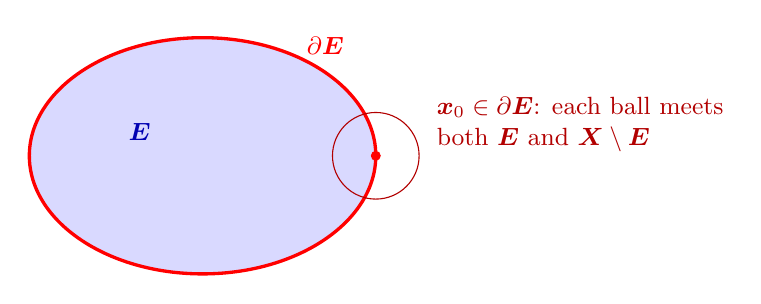
\begin{tikzpicture}[every node/.style={font=\small}]
	\fill[blue!15] (0,0) ellipse (2.2 and 1.5);
	\draw[red, very thick] (0,0) ellipse (2.2 and 1.5);
	\node[blue!70!black] at (-0.8,0.3) {$\boldsymbol{E}$};
	\node[red, anchor=west] at (1.2,1.4) {$\partial\boldsymbol{E}$};
	\fill[red] (2.2,0) circle (1.8pt);
	\draw[red!70!black] (2.2,0) circle (0.55);
	\node[red!70!black, anchor=west, align=left] at (2.85,0.4) {$\boldsymbol{x}_0\in\partial\boldsymbol{E}$: each ball meets\\ both $\boldsymbol{E}$ and $\boldsymbol{X}\setminus\boldsymbol{E}$};
\end{tikzpicture}
\end{document}
